\documentclass[ceqn,10pt]{SelfArx} 
\usepackage[spanish]{babel}
\selectlanguage{spanish} 
\usepackage[spanish,onelanguage]{algorithm2e}
%----------------------------------------------------------------------------------------
%	COLUMNS
%----------------------------------------------------------------------------------------

\setlength{\columnsep}{0.55cm} 
\setlength{\fboxrule}{0.75pt}
\usepackage{lipsum} % Required to insert dummy text. To be removed otherwise
\usepackage{amsmath}
\usepackage{algorithm}
\usepackage{algorithmic}
\usepackage{xcolor}
\makeatletter
\renewcommand{\ALG@name}{Pseudo-Código}

\makeatother
\graphicspath{ {./Imagenes/} } 


%----------------------------------------------------------------------------------------
%	COLORS
%----------------------------------------------------------------------------------------

\definecolor{color1}{RGB}{0,0,0} % Color of the article title and sections
\definecolor{color2}{RGB}{230, 231, 231} % Color of the boxes behind the abstract and headings
\definecolor{color3}{RGB}{0,0,0}
%----------------------------------------------------------------------------------------
%	HYPERLINKS
%----------------------------------------------------------------------------------------

\usepackage{hyperref} % Required for hyperlinks

\hypersetup{
	hidelinks,
	colorlinks,
	breaklinks=true,
	urlcolor=blue,
	citecolor=color1,
	linkcolor=color1,
	bookmarksopen=false,
	pdftitle={Title},
	pdfauthor={Author},
}

%----------------------------------------------------------------------------------------
%	ARTICLE INFORMATION
%----------------------------------------------------------------------------------------

\JournalInfo{Método de Muller, 2022} % Journal information
\Archive{Análisis numérico}
\PaperTitle{Método de Muller} % Article title

\Authors{Juan Páez\textsuperscript{1}, Santiago Zuñiga\textsuperscript{2}} % Authors
\affiliation{\textsuperscript{1}\textit{Facultad de ingeniería, Pontificia Universidad Javeriana}} % Author affiliation
\affiliation{\textsuperscript{2}\textit{Facultad de ingeniería, Pontificia Universidad Javeriana}} % Author affiliation
\affiliation{\textbf{Autor correspondiente}: jd.paez@javeriana.edu.co} % Corresponding author

\Keywords{Muller --- Solution --- Roots --- One Variable --- Error --- Polynomial\\
\textbf{Palabras clave} \\
Muller --- Solución --- Raíces --- Una Variable --- Error --- Polinimio}
% Keywords - if you don't want any simply remove all the text between the curly brackets
\newcommand{\keywordname}{Keywords} % Defines the keywords heading name

%----------------------------------------------------------------------------------------
%	ABSTRACT
%----------------------------------------------------------------------------------------

\Abstract{In this paper we will explain the Muller method used 
to solve equations in one variable with complex roots, we will also 
present an application problem with the computational solution and 
the respective error analysis.\\
\textbf{Resumen}\\ En este documento se explicará el método de Muller
usado para resolver ecuaciones en una variable con raíces complejas,
también presentaremos un problema de aplicación con su solución 
computacional y su respectivo análisis del error.
}

%----------------------------------------------------------------------------------------

\begin{document}
\renewcommand{\abstractname}{Abstract}
\maketitle % Output the title and abstract box

\thispagestyle{empty} % Removes page numbering from the first page

%----------------------------------------------------------------------------------------
%	ARTICLE CONTENTS
%----------------------------------------------------------------------------------------

\section*{Introducción} % The \section*{} command stops section numbering

\addcontentsline{toc}{section}{Introduction} % Adds this section to the table of contents
A la hora de solucionar ecuaciones no lineales en una variable, 
es decir encontrar o aproximar sus raíces, se pueden utilizar 
distintos métodos, como el despeje directo, Newton, posición falsa, 
entre otros. Sin embargo, se presenta un problema cuando las funciones que 
queramos evaluar tengan raíces complejas, ya que los métodos mencionados
no son los indicados para este tipo planteamientos. \\
Es por eso que el matemático estadounidense, David Eugene \textbf{Muller}, 
propuso un método para poder obtener una aproximación de este tipo de 
funciones el cual será explicado y desarrollado a lo largo de este documento.


%------------------------------------------------

\section{Definición}

El método de Muller, esta muy relacionado con el método de la secante, 
teniendo en cuenta que este consiste en tener una aproximación de la 
raíz a partir de dos puntos en la función $f(x)$. 

\begin{figure}[ht]\centering
	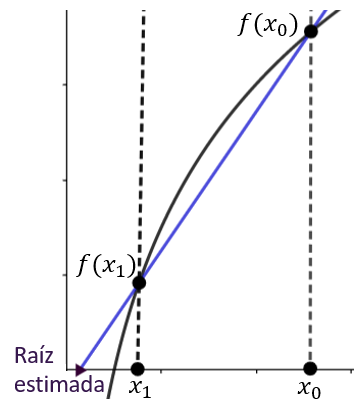
\includegraphics[scale=0.5]{GrafSecante.png}\\\ 
	\caption{Método de la secante}
	\label{fig:secante}
\end{figure}
En el caso de Muller consiste en tener 3 puntos 
sobre la gráfica de la función, siendo estos una 
composición cuadrática, la cual da una aproximación 
de la solución o raíz de $f(x)$.
\begin{figure}[ht]\centering
	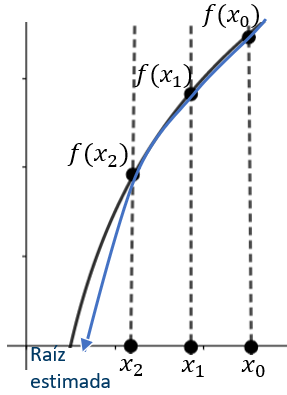
\includegraphics[scale=0.5]{GrafMuller.png}\\\
	
	\caption{Método de Muller}
	\label{fig:muller}
\end{figure}

\subsection{Definición matemática}

Teniendo en cuenta la forma general de la ecuación cuadrática y la aproximación de la raíz,
el metodo comienza planteando el siguiente polinomio cuadrático:
\begin{equation} \label{eq:formaGeneral}
	g(x)=a(x-x_{2})^2+b(x-x_{2})+c
\end{equation}
Queremos que la función $g(x)$, representada de color azul, 
pase por los puntos presentados en la figura \ref*{fig:muller},
es decir $[x_{0},f(x_{0})]$ , $[x_{1},f(x_{1})]$ y $[x_{2},f(x_{2})]$,

por lo tanto sustituyendo en la ecuación (\ref*{eq:formaGeneral}),
nos da las respectivas imagenes de las funciones en $g(x_{k})$.

\begin{equation} \label{eq:g0}
\begin{aligned}
	g(x_{0})=a(x_{0}-x_{2})^2+b(x_{0}-x_{2})+c
\end{aligned}
\end{equation}
\begin{equation} \label{eq:g1}
\begin{aligned}
	g(x_{1})=a(x_{1}-x_{2})^2+b(x_{1}-x_{2})+c
\end{aligned}
\end{equation}
\begin{equation} \label{eq:g2}
\begin{aligned}
	g(x_{2})=a(x_{2}-x_{2})^2+b(x_{2}-x_{2})+c
\end{aligned}
\end{equation}
Al haber tres ecuaciones, podemos hallar los valores de los tres coeficientes $a$, $b$ y $c$.
Empezando por el valor de $c$, que utilizando la ecuación (\ref*{eq:g2}) sería:
\begin{equation} \label{eq:g2S}
	\begin{aligned}
	g(x_{2})=a(0)^2+b(0)+c\\
	g(x_{2})=c
\end{aligned}
\end{equation}
Por lo tanto al reemplazar $c$ en las ecuaciones (\ref*{eq:g0}) y (\ref*{eq:g1}) tenemos que:
\begin{equation} \label{eq:despejeg0}
	\begin{aligned}
	g(x_{0})-g(x_{2})=a(x_{0}-x_{2})^2+b(x_{0}-x_{2})
\end{aligned}
\end{equation}
\begin{equation} \label{eq:despejeg1}
	\begin{aligned}
	g(x_{1})-g(x_{2})=a(x_{1}-x_{2})^2+b(x_{1}-x_{2})
\end{aligned}
\end{equation}
Empleando la fórmula para hallar la pendiente de una recta, podemos hallar
una aproximación a las derivadas, dando como resultado
los coeficientes $a$ y $b$.
\begin{equation} \label{eq:ecuacionesPendiente}
	\begin{aligned}
	h_{0}=x_{1}-x_{0}\\
	h_{1}=x_{2}-x_{1}
\end{aligned}
\end{equation}
\begin{equation} \label{eq:deltas}
	\begin{aligned}
	\delta_{0}= \frac{f(x_{1})-f(x_{0})}{x_{1}-x_{0}}\\
	\delta_{1}= \frac{f(x_{2})-f(x_{1})}{x_{2}-x_{1}}
\end{aligned}
\end{equation}
Utilizando las ecuaciones (\ref*{eq:deltas}) y
(\ref*{eq:ecuacionesPendiente}), reemplazándolas en (\ref*{eq:despejeg0}) y
(\ref*{eq:despejeg1})
\begin{equation} \label{eq:reemp}
	\begin{aligned}
	 h_{0}\delta_{0}+h_{1}\delta_{1} = b(h_{0}+h_{1})-a(h_{0}+h_{1})^2\\
	 h_{1}\delta_{1} = b h_{1} - ah_{1}^2 
\end{aligned}
\end{equation}
Al despejar $a$ y $b$, de la anterior ecuación nos da el resultado de los coeficientes
\begin{equation} \label{eq:coeficienteA}
	\begin{aligned}
	a = \frac{\delta_{1}-\delta_{0}}{h_{1}-h_{0}}
\end{aligned}
\end{equation}
\begin{equation} \label{eq:coeficienteB}
	\begin{aligned}
	b = a h_{1} + \delta_{1}
\end{aligned}
\end{equation}
Teniendo como calcular los coeficientes, podemos hallar la raíz $x_{3}$ por
medio de la fórmula cuadrática en (\ref*{eq:formaGeneral}) con $x = x_{3}$,
sin embargo, como se comenta en las referencias
\cite{burden2017, chapra2011}, no se puede emplear la formula tal cual, teniendo en cuenta
los posibles errores de redondeo al usarla, por lo tanto hay que usar una
variante:
\begin{equation} \label{eq:x3}
	\begin{aligned}
	x_{3}-x_{2}=\frac{-2c}{b (signo(b))\sqrt{b^2-4ac}}
\end{aligned}
\end{equation}
Despejando $x_{3}$
\begin{equation} \label{eq:x3Solv2}
	\begin{aligned}
	x_{3}=\frac{-2c}{b(signo(b))\sqrt{b^2-4ac}}+x_{2}
\end{aligned}
\end{equation}
Teniendo en cuenta que $x_{2}$ de manera iterativa es el punto más
aproximado a la raíz, el error se calcula:
\begin{equation} \label{eq:error}
	\begin{aligned}
	\epsilon_{n}= |\frac{x_{3}-x_{2}}{x_{3}}|
\end{aligned}
\end{equation}

Cabe mencionar que el signo que se escoge para este método, en la variante
de la formula cuadrática, es el mismo signo de $b$, para que el denominador
sea más grande, dando un número más aproximado a la raíz, por eso se usa la
notación $signo(b)$.
\section{Pseudo-Código}
A continuación se presenta como sería la implementación del método,
expresado en palabras naturales:\\\
\begin{algorithm}[H] %or another one check
 \caption{Muller}
 \textbf{Requiere:} $x_{0}$, $x_{1}$, $x_{2}$, $f(x)$ (Función a evaluar), $iter$ (Iteraciones máximas), $tol$ (Tolerancia del error).\\
 \textbf{Salida:} Aproximación de la raíz, con cuantas iteraciones.\\
     \SetAlgoLined
     \While{$i < iter$ }{
      {\color{violet}\CommentSty{Calcular:}}\\
      $h_{0} = x_{1}-x_{0}$\\
      $h_{1} = x_{2}-x_{1}$\\
      $d_{0}= (f(x_{1})-f(x_{0}))/h_{0}$\\
	  $d_{1}= (f(x_{2})-f(x_{1}))/h_{1}$\\
	  \\
	  {\color{violet}\CommentSty{Calcular a b y c }}\\
	  \state $a = d_{1}-d_{0}/h_{1}+h_{0}$\\ 
	  $b = ah_{1} + d_{1}$
	  \\
	  $c = f(x_{2})$\\
	  \\
	  {\color{violet}\CommentSty{Calcular denominador más grande}}\\
	  \state $rad = \sqrt{b^{2}-4ac}$\\
	  \eIf{$|b+rad| > |b-rad|$}{ 
	   $deno = b+rad$
	   }{
	   $deno = b-rad$
	   }\\
	   \\
	   {\color{violet}\CommentSty{Encontrar $x_{3}$}} \\
	   $x_{3} = x_{2} + (-2c)/deno$\\
	   \\
	   {\color{violet}\CommentSty{Calculo del error} }\\
	   \eIf{$|x_{3}-x_{2}| < tol$ }{\\
	   \\
	        \textbf{retorne} $x_{3},i$
	    }{
	    {\color{violet}\CommentSty{Siguiente iteración}}\\
	        $x_{0} = x_{1}$\\
	        $x_{1} = x_{2}$\\
	        $x_{2} = x_{3}$
	    }
      \\
      \\
      $i = i +1$
     }
     \textbf{Imprimir } No se pudo llegar a una solución con la tolerancia requerida\\
     \textbf{retorne} $x_{3},i$\\
\end{algorithm}
Ahora que ya se definió como es el algoritmo del método de Muller, a
continuación se presentará un problema extraído del libro de Burden, el
cual será solucionado a partir de un algoritmo desarrollado en lenguaje de
programación \emph{Python}.
\section{Problema de aplicación}
El problema a evaluar es de la sección 2.6, ejercicio numero
10\cite{burden2017}:
\begin{figure}[ht]\centering
	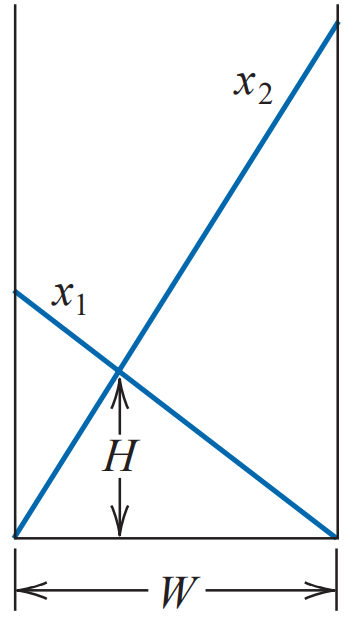
\includegraphics[scale=0.4]{problema.png}\\\
	\caption{Dibujo problema}
	\label{fig:problema}
\end{figure}
\\Dos escaleras atraviesan un callejón de ancho $w$. Cada escalera llega
desde la base de una pared hasta algún punto de la pared opuesta. Las
escaleras se cruzan a una altura H sobre la acera. Halla W dado que las
longitudes de las escaleras son $x_{1} = 20$ pies y $x_{2} = 30$ pies, y
que $H = 8$ pies.\\
\section{Planteamiento del problema}
\begin{figure}[ht]\centering
	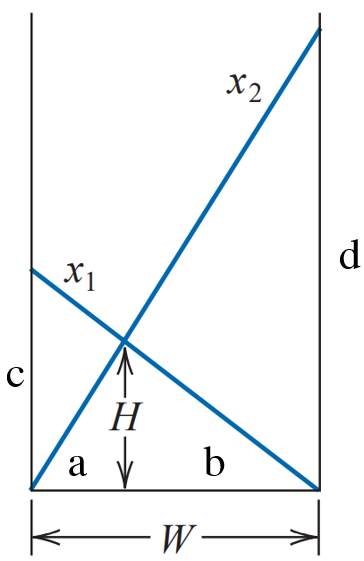
\includegraphics[scale=0.4]{planteamiento.png}\\\
	\caption{Planteamiento problema}
	\label{fig:planteamiento}
\end{figure}
Empezamos creando unas nuevas variables, siendo $a$ la distancia de la pared
de la izquierda hasta donde se cruzan las escaleras, y $b$ es parecido la
distancia de $a$, solo que lo mide desde el cruce hasta la pared de la
derecha. Con $c$, se crea un triangulo rectángulo entre $w$ y
$x_{1}$, y con $d$ se crea otro triangulo de noventa grados con $w$ y
$x_{2}$\\
Por el teorema de pitágoras
\begin{equation} \label{eq:pitagoras}
\begin{aligned}
	w^2+c^2=x_{1}^2\\
	w^2+d^2=x_{2}^2
\end{aligned}
\end{equation}
Despejando $c$ y $d$ tenemos
\begin{equation} \label{eq:pitagoras2}
\begin{aligned}
	c=\sqrt{x_{1}^2-w^2}\\
	d=\sqrt{x_{2}^2-w^2}
\end{aligned}
\end{equation}
Siguiendo con el teorema de tales
\begin{equation} \label{eq:tales}
\begin{aligned}
	\frac{a}{h} = \frac{w}{d}\\
	\\
	\frac{b}{h} = \frac{w}{c}
\end{aligned}
\end{equation}
Reemplazando (\ref{eq:pitagoras2}) y despejando $a$ y $b$ en la anterior ecuación
\begin{equation} \label{eq:despejeTales}
\begin{aligned}
	a = \frac{w \cdot h}{\sqrt{x_{2}^2-w^2}}\\
	b = \frac{w \cdot h}{\sqrt{x_{1}^2-w^2}}
\end{aligned}
\end{equation}
Sabemos entonces, que la suma de $a$ y $b$ da la distancia de $w$, entonces,
usando (\ref{eq:despejeTales}) tenemos
\begin{equation} \label{eq:obtenerW}
\begin{aligned}
	w = \frac{w \cdot h}{\sqrt{x_{2}^2-w^2}} + \frac{w \cdot h}{\sqrt{x_{1}^2-w^2}}
\end{aligned}
\end{equation}
Moviendo $w$ al otro lado de la ecuación tenemos que
\begin{equation} \label{eq:ecuacionW}
\begin{aligned}
	1 = \frac{h}{\sqrt{x_{2}^2-w^2}} + \frac{h}{\sqrt{x_{1}^2-w^2}}
\end{aligned}
\end{equation}
Reemplazando $h$, $x_{1}$ y $x_{2}$ da la ecuación
\begin{equation} \label{eq:despejeW}
\begin{aligned}
	0 = \frac{8}{\sqrt{30^2-w^2}} + \frac{8}{\sqrt{20^2-w^2}}-1
\end{aligned}
\end{equation}
Esta sería la respuesta final de la solución del problema, sin embargo, este método
debe ser empleado solo con polinomios, por lo tanto, hay que deshacerse de esos
radicales, entonces luego de unos operaciones algebraicas, la ecuación expresada como
de la manera correcta es
\begin{equation} \label{eq:despejeW}
\begin{aligned}
	(400-w^2)^2 (230400-256w^2)-\\
(57600-64 w^2-964 (400-w^2)+w^2 (400-w^2))^2
\end{aligned}
\end{equation}
\section{Solución con implementación}
Usando el programa desarrollado en \emph{Python}, con la 
implementación del método de la secante obtenido de internet y escogiendo
 a $x_{0}$, $x_{1}$ y $x_{2}$, a partir del método gráfico \cite{gg2} 
 \begin{figure}[ht]\centering
	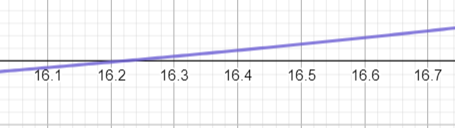
\includegraphics[scale=0.6]{graficoEcuacion.png}\\\
	\caption{Raíz de la ecuación}
	\label{fig:raicesGraf}
\end{figure}\\
 Nos da como resultado, con sus respectivas iteraciones
\begin{figure}[ht]\centering
	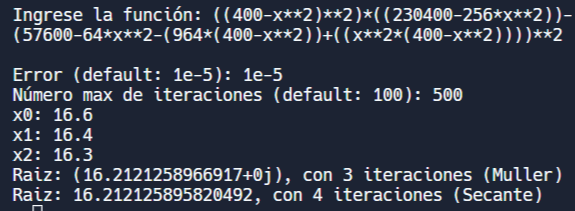
\includegraphics[scale=0.5]{solucionPython.png}\\\
	\caption{Salida solución programa}
	\label{fig:fotoPython}
\end{figure}\\
Utilizando la herramienta Wolfram Alpha \cite{wolfram}, podemos
evidenciar cual es la raíz exacta, dándonos como resultado
\begin{equation} \label{eq:wolfram}
\begin{aligned}
	x \approx 16.21212589669170009828922\notag
\end{aligned}
\end{equation}
Mostrando que los dos métodos pudieron obtener la
aproximación de la  raíz, sin embargo, el método de Muller 
tuvo una convergencia más rápida haciéndolo en una iteración menos que el de la Secante.
\section{Conclusión}
Como se mencionó al principio del documento, este método es bastante útil
para poder encontrar raíces complejas, por el hecho de que usa la formula cuadrática,
facilitando a si mismo, el manejo de este tipo de soluciones, y, aunque la secante también
funciona para este tipo de problemas, lo que buscamos en el \textit{Análisis numérico}
es que la convergencia a la aproximación de la raíz sea con las menos iteraciones posibles
minimizando el error, es por eso que lo ideal para este tipo de ecuaciones es usar el método
propuesto por David.
\phantomsection
\bibliographystyle{unsrt}
\bibliography{referencias.bib}

\end{document}
